c\renewcommand{\chaptername}{Capitulo}
\chapter{Marco Teórico} 
\section{Metadatos}

Hoy día, gran cantidad de información existe sobre cualquier tipo de temas en la red, sin embargo, lo realmente importante es la cantidad de servicios disponibles para los usuarios para poder acceder a ésta información desde cualquier lugar y mediante cualquier dispositivo. A lo largo de los años, la cantidad de información ha crecido de tal manera que es fácil perderse en ese universo alterno en que todos de alguno u otra manera estamos inmersos. No obstante, aunado al problema inherente del tamaño, la falta de etiquetado de los contenidos en la web se traducen en mayor esfuerzo para la recuperación de información.\newline

El etiquetado de contenidos juega un papel crucial ya que permite una adecuada categorización, además de la descripción necesaria para que las páginas web se localicen y procesen adecuadamente por un agente (computadora, aplicación o programa). Según \cite{W3C}, una prioridad particular de W3C es usar la Web para documentar el significado de los metadatos. El gran interés en los metadatos ha impulsado el desarrollo del Marco de Descripción de Recursos (RDF) donde aún hay un gran campo de trabajo sin explorar.\newline



\section{Resource Description Framework - RDF}

La \textit{World Wide Web} o también conocida simplemente como \textit{Web} es una plataforma tecnológica la cual constituye la mayor base de datos existente, conformada por todo tipo de recursos, donde una persona o también llamada usuario, puede publicar, explorar, consultar o guardar información.\newline

Sin embargo, inicialmente la Web sólo almacenaba recursos informáticos entendibles para los seres humanos sin considerar que, con el paso del tiempo sería de suma importancia automatizar el tratamiento de los mismos a través de computadoras. Por lo anterior, la Web semántica promueve el modelado, etiquetado y representación de la información de tal manera que, ahora tanto los humanos, como las computadoras sean capaces \textit{comprender} el contenido de una página o recurso almacenado en la Web.

\begin{figure}[!ht]
    \centering
    \includegraphics[width=10cm]{figures/Modelo_capas_web_semantica.jpg} %NOMBRE DE LA FIGURA y TAMAÑO
    \caption{Modelo de capas de Berners-Lee para la web semántica\cite{WebSemantica_SciELO}} %PIE DE LA IMAGEN
    \label{Modelo_Web_Semantica}
\end{figure}

En ese sentido, la Web semántica como se menciona en \cite{IntroBD_RDF}, propone una alternativa que agrega significado a los contenidos almacenados en la Web, lo cual permite una interacción más fluida entre aplicaciones, servicios o computadoras y el ser humano. Para ello, es necesario trabajar bajo ciertas normas o lenguajes estándar organizados en capas o niveles, como se muestra en la figura \ref{Modelo_Web_Semantica}, los cuales se describen a continuación: \cite{IntroBD_RDF}

\begin{itemize}
    \item \textit{Unicode} \cite{W3C}. Estándar para documentos de texto que permite codificar la mayoría de los sistemas de escritura del mundo.
    
    \item \textit{URI\footnote{\textit{Uniform resource identifier} (Identificador uniforme de recursos)}} \cite{W3C}. Estándar para crear identificadores de recursos Web a través de cadenas compactas de caracteres que permititen su identificación unívoca y localización automática. Una URL\footnote{\textit{Uniform resource locator} (identificador de recursos uniforme)} es un ejemplo de una URI, como \texttt{http://informatica.uppuebla.edu.mx/~mmedina/} puede ser usado para identificar específicamente un recurso, es éste caso a una persona dentro de un site institucional.
    
    \item \textit{XML\footnote{\textit{Extensible markup language} (Lenguaje de Marcado Extensible o Lenguaje de Marcas Extensible)}} \cite{W3C}. Es un lenguaje de marcado similar a HTML y es una especificación de W3C\footnote{\textit{World Wide Web Consortium} (Consorcio WWW)} como lenguaje de marcado de propósito general, es decir que, no está predefinido, por lo que es necesario definir sus propias etiquetas. 
    
    \item \textit{XML Namespaces} (Espacios de nombre de XML) \cite{W3C}. Es una recomendación W3C, la cual a través de etiquetas se califican y clasifica los términos de un documento XML, de tal manera que cada término esta identificado por una URI que lo hace único y universal, evitando así la ambigüedad de los documentos en la Web.
    
    \item \textit{RDF}\footnote{\textit{Resource Description Framework} (Marco de descripción de recursos)} \cite{W3C_SemanticWeb}. Modelo estándar para el intercambio de datos en la Web, con características que facilitan la fusión de datos inclusive si los esquemas subyacentes son diferentes. Además, RDF amplía la estructura de enlace de la Web para utilizar los URI para nombrar la relación entre las cosas, así como los dos extremos del enlace (esto generalmente se conoce como un \textit{terna}). A través de este modelo es posible que datos estructurados y semiestructurados se puedan mezclar, compartirse y consumirse por diferentes aplicaciones.
    
    \item \textit{RDF Schema} \cite{W3C_RDFSchema}. Proporciona un vocabulario de modelado de datos para RDF, complementandose con diferentes documentos anexos que describen los conceptos básicos y la sintaxis abstracta de RDF. Es una extensión semántica de RDF que proporciona mecanismos para describir grupos de recursos relacionados y las relaciones entre estos recursos. El esquema RDF está escrito en RDF usando los términos descritos en este documento. Estos recursos se utilizan para determinar las características de otros recursos, como los dominios y los rangos de propiedades.
    
    \item \textit{Ontología}. 
    
    \item \textit{Capa lógica}.
    
    \item \textit{Capa de prueba}.
    
    \item \textit{Capa de confianza}.

\end{itemize}

Considerando lo anterior, la mayoría de los elementos semánticos descritos en la Web se encuentran en formatos XML, RDF y OWL.\newline


\section{SPARQL}

Como ya se mencionó, RDF es un formato de datos que puede ser representado como un modelo de grafos dirigidos etiquetados, que representan información en la Web. Además de otros usos, como la representación de información personal, redes sociales, metadatos sobre objetos digitales y un medio para la integración de fuentes de información heterogeneas, donde SPARQL\footnote{\textit{SPARQL PROTOCOL AND RDF QUERY LANGUAGE} (Protocolo y lenguaje de consulta para RDF)} es un lenguaje de consulta para los formatos RDF.\newline

Según \cite{Skos_Sparql}, el lenguaje SPARQL cuenta con las siguientes especificaciones:

\begin{itemize}
    \item La especificación del Protocolo SPARQL para RDF [SPROT] que define el protocolo remoto para enviar consultas SPARQL y recibir los resultados.
    \item La especificación del Formato XML de los resultados de consultas SPARQL [RESULTS] que define un formato de documento XML para representar los resultados de las consultas SELECT y ASK de SPARQL.
\end{itemize}

Por lo anterior, se puede identificaf que SPARQL es tanto un protocolo, como un lenguaje de consulta para RDF basados en estandares de 3WC. Esta orientado a datos ya que sólo extrae la información contenida en el modelo ontológico y devuelve resultados en forma de enlaces o en esquemas RDF.\newline

La figura \ref{ejemplo_RDF_grafico} muestra una representación gráfica simple de \textit{vc-db-1.rdf}, archivo que contiene RDF para varias descripciones de vCard de personas, descritas en las notas del W3C "Representación de objetos vCard en RDF / XML".\newline

\begin{figure}[!ht]
    \centering
    \includegraphics[width=10cm]{figures/vc-db.png} %NOMBRE DE LA FIGURA y TAMAÑO
    \caption{Ejemplo de representación gráfica provenientes de Representación de objetos vCard en RDF / XML} %PIE DE LA IMAGEN
    \label{ejemplo_RDF_grafico}
\end{figure}

La figura \ref{ejemplo_RDF_ternas} muestra el esquema RDF expresado como un conjunto de ternas (también llamadas tripletas).\newline

\begin{figure}[!ht]
    \centering
    \includegraphics[width=10cm]{figures/ejemplo_RDF.jpg} %NOMBRE DE LA FIGURA y TAMAÑO
    \caption{Ejemplo de conjunto de ternas en RDF} %PIE DE LA IMAGEN
    \label{ejemplo_RDF_ternas}
\end{figure}
    


\section{Servicios REST}

Los servicios REST formaron una gran opción para la explotación de recursos apartir de la migración a la web 2.0, sustitutendo aquellos que hacian uso de los protocolos SOAP y WSDL, haciendo uso de una arquitectura más sencilla, orientado a recursos y haciendo uso del protocolo HTTP. Los servicios REST \footnote{\textit{Representational State Transfer} (Transferencia de Estado Representacional)} cumplen con las siguientes premisas: \cite{FeaturesREST}

\begin{itemize}
    \item Se define una \textbf{interfaz} de comunicación \textbf{cliente-servidor} separando completamente las responsabilidades entre ambas partes, como se muestra en la figura \ref{arquitectura_REST_1}.
    
    \begin{figure}[!ht]
    	\centering
    	\includegraphics[width=10cm]{figures/Cliente_servidor_REST.png} %NOMBRE DE LA FIGURA y TAMAÑO
        \caption{Arquitectura cliente servidor de servicio REST} %PIE DE LA IMAGEN
        \label{arquitectura_REST_1}
    \end{figure}
    
    \item Servicio web \textbf{sin estado} ya que  cada petición que se realiza es completamente independiente de cualquier otra, sin embargo, todas las solicitudes al mismo servicio son totalmente idénticas, como se muestra en la figura \ref{arquitectura_REST_2}.
    
    \begin{figure}[!ht]
    	\centering
    	\includegraphics[width=10cm]{figures/Cliente_servidor_REST_2.png} %NOMBRE DE LA FIGURA y TAMAÑO
        \caption{Servicios sin estado de la Arquitectura cliente servidor REST} %PIE DE LA IMAGEN
        \label{arquitectura_REST_2}
    \end{figure}
    
    \item Los servicios web REST pueden guardar en cache su contenido de tal manera que una vez realizada la primera petición al servicio, el resto de peticiones puedan apoyarse en la cache si fuera necesario, como se muestra en la figura \ref{arquitectura_REST_3}.
    
    \begin{figure}[!ht]
    	\centering
    	\includegraphics[width=10cm]{figures/Cliente_servidor_REST_3.png} %NOMBRE DE LA FIGURA y TAMAÑO
        \caption{Servicios REST apoyados en cache} %PIE DE LA IMAGEN
        \label{arquitectura_REST_3}
    \end{figure}
    
    \item Todos lo servicios REST son \textbf{uniformes}, es decir, que compartirán una forma de invocación y métodos similares utilizando los metodos GET,POST,PUT ,DELETE, como se muestra en la figura \ref{arquitectura_REST_4}.
    
    \begin{figure}[!ht]
    	\centering
    	\includegraphics[width=10cm]{figures/Cliente_servidor_REST_4.png} %NOMBRE DE LA FIGURA y TAMAÑO
        \caption{Servicios REST uniformes} %PIE DE LA IMAGEN
        \label{arquitectura_REST_4}
    \end{figure}
    
    \item Finalmente, todos los servicios REST son escalables y para el cliente REST es transparente, es decir, no será capaz de distinguir entre si la petición es atendida directamente por servidor , o por el sistema de caches, a través de un servicio de balanceo de cargas, como se muestra en la figura \ref{arquitectura_REST_5}.
    
    \begin{figure}[!ht]
    	\centering
    	\includegraphics[width=10cm]{figures/Cliente_servidor_REST_5.png} %NOMBRE DE LA FIGURA y TAMAÑO
        \caption{Arquitectura de capas de los Servicios REST} %PIE DE LA IMAGEN
        \label{arquitectura_REST_5}
    \end{figure}
    
\end{itemize}

Si bien algunos repositorios institucionales (RIs) cuentan con servicios tipo REST , el grado de complejidad en las consultas que hasta el momento estan implementadas, consideran sólo un atributo, lo cual restringe el tipo de información que puede recuperarse.\newline

En ese sentido, el RN ofrece a sus usuarios un catálogo abierto con más de doscientos servicios REST que estan disponibles para todos los usuarios que soliciten información en formato JSON de diversos catálogos, como se puede consultar en \cite{CatalogoREST_RN}. La descripción general se muestran a continuación en el cuadro \ref{descripcion_servicios_REST_RN}.

\begin{table}[!ht]
    \centering
    \includegraphics[width=10cm]{figures/Tabla_servicios_REST.png} %NOMBRE DE LA FIGURA y TAMAÑO
    \caption{Descripción de los servicios REST ofrecidos por el RN} %PIE DE LA IMAGEN
    \label{descripcion_servicios_REST_RN}
\end{table}

Para que un usuario pueda consultar alguno de los catálogos de datos, es necesario identificar la búsqueda concreta que arroje la información que se desea consultar. Al mismo tiempo, existen al menos sietes servicios básicos de consulta y otros más específicos, dependiendo del catálogo. Un ejemplo de lo anterior se muestra en la figura \ref{ejemplo_consumo_REST_RN}.

\begin{figure}[!ht]
    \centering
    \fbox{
    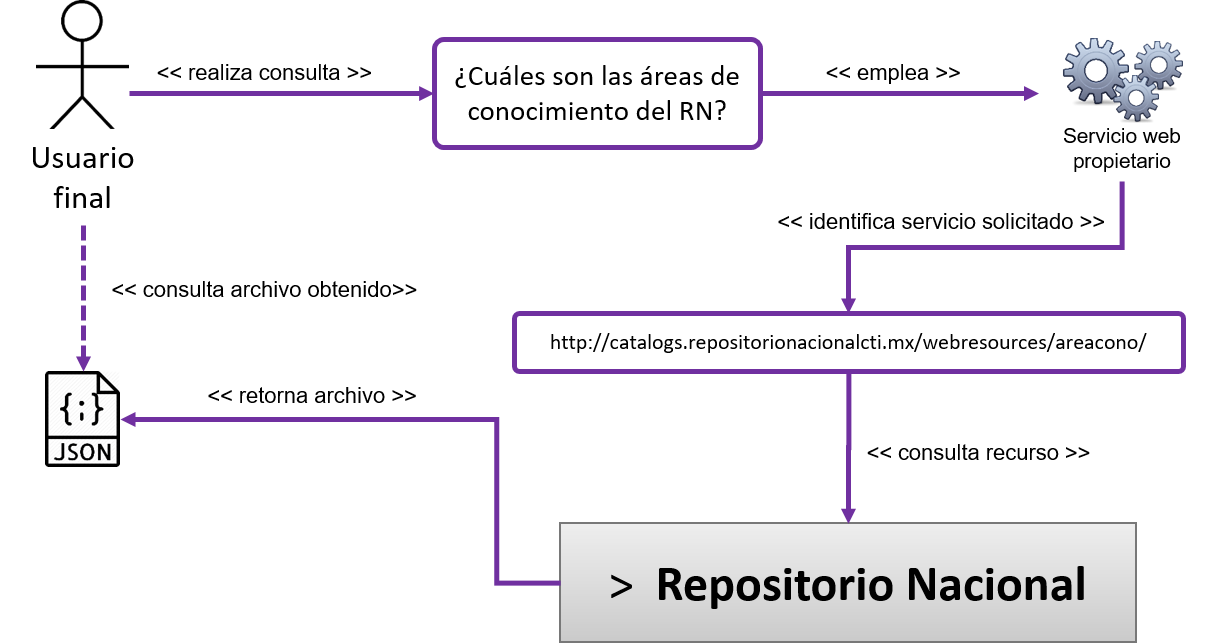
\includegraphics[width=12cm]{figures/ConsumoREST.png}} %NOMBRE DE LA FIGURA y TAMAÑO
    \caption{Ejemplo de consumo de un servicio REST del RN} %PIE DE LA IMAGEN
    \label{ejemplo_consumo_REST_RN}
\end{figure}

Finalmente, el resultado de la consulta efectuada mediante uno de los servicios REST, es un archivo en formato JSON \footnote{JSON o \textit{JavaScript Object Notation} es un  formato de texto ligero para el intercambio de datos}, como se observa en la figura \ref{JSON_ejemplo_consumo_REST_RN}.

\begin{figure}[!ht]
    \centering
    \fbox{
    \includegraphics[width=12cm]{figures/JSON_servicio_REST_RN.png}} %NOMBRE DE LA FIGURA y TAMAÑO
    \caption{Archivo tipo JSON obtenido mediante servicio REST del RN} %PIE DE LA IMAGEN
    \label{JSON_ejemplo_consumo_REST_RN}
\end{figure}

\section{COAR}

En 2016, la Confederation of Open Access Repositories - \textit{COAR} (Confederación de Repositorios de Acceso Abierto) integró un equipo de trabajo llamado \textit{Next Generation Repository Working Group} (Equipo de trabajo para la siguiente generación de repositorios) cuyo porpósito fue el de definir las funcionalidades y tecnologías a desarrollar en los RDs en los próximos años. Derivado de estos trabajos, el informe \textit{Behaviours and Technical Recommendations of the COAR Next Generation Repositorie} \cite{NextGenerationRepositories} indicó que será necesario adoptar nuevas tecnologías, estándares y protocolos que permitan una mejor integración de los repositorios en los entornos web, de esta manera, éstos jugarán un papel importante en el amplio campo de la comunicación académica.

Lo anterior dejó al descubierto que, hoy en día muchas de los medios de difusión de la investigación y de la producción académica de las IES y CI, han cubierto estas funcionalidades desde un punto de vista básico, lo cual dista de ser lo ideal si lo que se pretende es darle covertura amplia y pertinente del los contenidos de los repositorios. Uno de los aspectos que no aportan a la igualdad y libre acceso a la información, es la publicación en medios tradicionales, cuyos incentivos coorporativos ponen en desventaja a aquellos que no cuentan con acceso a sus plataformas, medios digitales o impresos.

Finalmente, el estudio plantea once características importantes que los repositorios del futuro deben contemplar para establecerse como una fuente sólida de publicación, confiable y de AA: \cite{NextGenerationRepositories}

\begin{itemize}
\item Exponer \textit{identificadores}
\item Declaración de \textit{licencias} a nivel de recursos
\item Descubrimientos a través de la \textit{navegación}
\item Interactuar con \textit{recursos}
\item Descrubrimiento de \textit{lotes}
\item \textit{Transferencia} de recursos
\item \textit{Metadatos} de la actividad de recopilación y exposición de la información
\item \textit{Identificación} del usuario
\item \textit{Autenticación} del usuario
\item Exponer \textit{métricas} de uso estandarizadas
\item \textit{Conservación} de los recursos
\end{itemize}

La visión general del informe marca que, se deben establecer comunidades de investigadores y académicos que, por un lado, aporten al acervo de los repositorios, por otro lado, que al mismo tiempo incentiven la producción en su comunidad o en otras comunidades interesadas en participar, de tal manera que los repositorios brinden una visión global de la investigación científica y académica a través de plataformas tecnológicas o repositorios.

Por otro lado, el uso del protocolo \textit{Representational State Transfer} (REST) o protocolo de transferencia de estado representacional permite el intercambio y manipulación de datos a través de Internet, lo cual ayuda en el desarrollo de diversas aplicaciones y servicios web haciendo uso de datos con diversos orígenes. Empresas como Twitter, YouTube, Facebook, entre otras, han basado su operación en la implementación de servicios REST, presentado un crecimiento horizontal de manera acelerada.

REST funge como interfaz entre un RI que use HTTP para obtener datos o generar operaciones sobre esos datos en formatos como XML y JSON. De esta manera, se constituye como una alternativa en auge en comparación con otros protocolos estándar de intercambio de datos como \textit{Simple Object Access Protocol} (SOAP), que disponen de una gran capacidad pero también mucha complejidad, mientras que REST es una solución más sencilla y flexible para tales fines.

Algunas de las características mas relevantes de REST son las siguientes: ----- falta anexar

\begin{figure}[!ht]
	\centering
	\fbox{
	\includegraphics[width=10cm]{Arquitectura_Servicio_Web.png}} %NOMBRE DE LA FIGURA y TAMAÑO
    \caption{Arquitectura de servicio web semántico} %PIE DE LA IMAGEN
    \label{arquitect1}
\end{figure}


\section{UML}

UML\footnote{\textit{UML - Unified Modeling Language (Lenguaje de Modelado Unificado)}} es un lenguaje de modelado de sistemas utilizado ampliamente. Mediante una serie de herramientas gráficas permite visualizar, especificar, construir y documentar un sistema, en otras palabras, permite conformar el plano de un proyecto de software.\newline

UML se compone de una serie de herramientas o diagramas que sirven para modelar dos tipos de aspectos: \textit{estructura} y \textit{comportamiento}, como se muestra en la figura \ref{diagramas_UML}.

\begin{figure}[!ht]
    \centering
    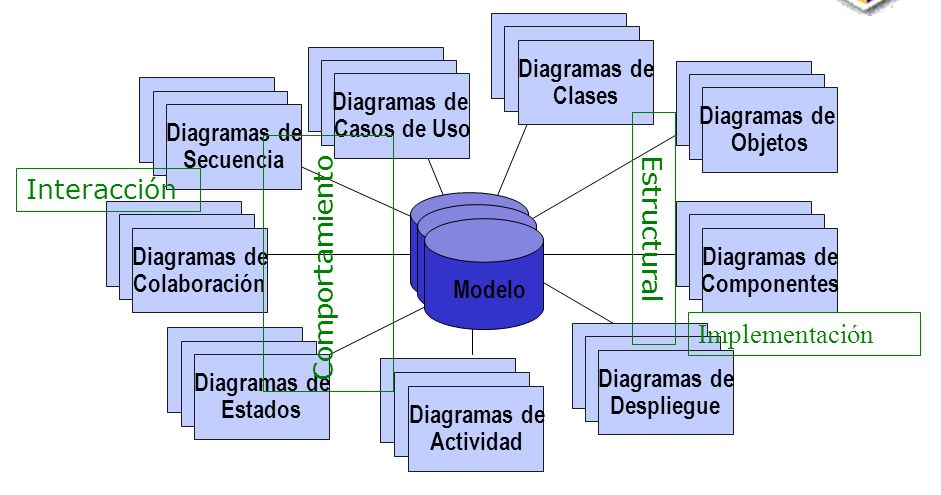
\includegraphics[width=10cm]{figures/diagramas_UML.png} %NOMBRE DE LA FIGURA y TAMAÑO
    \caption{Diagramas UML (Fuente: https://slideplayer.es/slide/151110/)} %PIE DE LA IMAGEN
    \label{diagramas_UML}
\end{figure}

\subsection{Diagrama de casos de uso}

Como punto de partida para el desarrollo del servicio web, se plantea el uso de dos herramientas básicas: el diagrama de \textit{casos de uso}, que ofrece una visión general de los involucrados (actores) en un sistema, las funciones que éstos realizan y cómo interactúan con las demás, y los principales procesos del sistema.\newline

\begin{figure}[!ht]
    \centering
    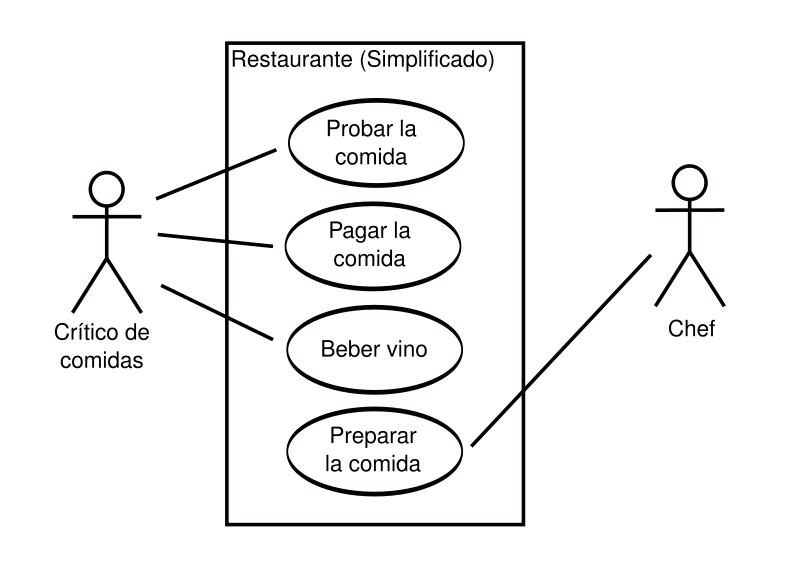
\includegraphics[width=10cm]{figures/diagrama_caso_de_uso.png} %NOMBRE DE LA FIGURA y TAMAÑO
    \caption{Ejemplo de diagrama de caso de uso (Fuente: https://es.wikipedia.org/wiki/Diagrama_de_casos_de_uso)} %PIE DE LA IMAGEN
    \label{diagrama_caso_de_uso}
\end{figure}

\subsection{Diagrama de clases}

La otra herramienta propuesta es un \textit{diagrama de clases}, el cual es un bloque de construcción principal de la solución orientada a objetos, donde se muestran las clases del servicio, sus atributos y métodos, además de las relaciones entre clases representadas con flechas.

\begin{figure}[!ht]
    \centering
    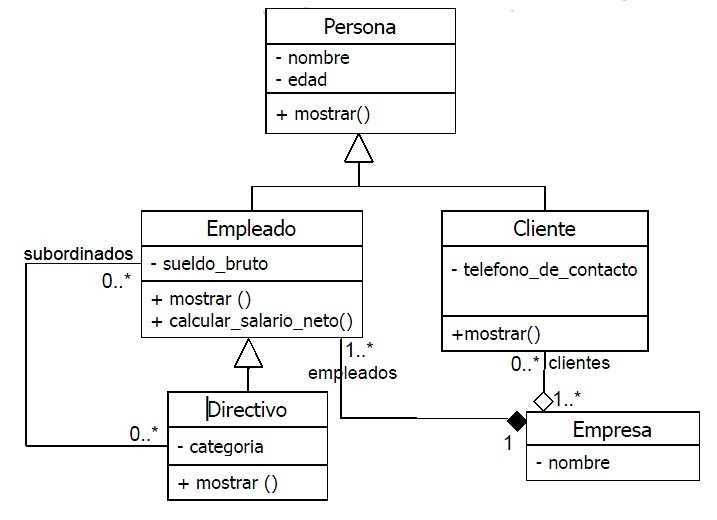
\includegraphics[width=10cm]{figures/diagrama_clases.jpg} %NOMBRE DE LA FIGURA y TAMAÑO
    \caption{Ejemplo de diagrama de clases (Fuente: https://sites.google.com/site/todouml/home)} %PIE DE LA IMAGEN
    \label{diagrama_clases}
\end{figure}

\section{Patrones de diseño *}

 Los patrones de diseño son estrategias independientes del lenguaje para resolver problemas comunes de diseño orientados a objetos. Cuando realice un diseño, debe saber los nombres de algunas soluciones comunes. Aprender patrones de diseño es bueno para que las personas se comuniquen entre sí de manera efectiva. De hecho, es posible que haya estado familiarizado con algunos patrones de diseño, y que no utilice nombres conocidos para describirlos. SUN sugiere GOF (Gang Of Four: cuatro chicos pioneros que escribieron un libro llamado "Patrones de diseño" - Elementos de software orientado a objetos reutilizables), por lo que usamos ese libro como nuestra guía para describir las soluciones. Por favor, familiarícese con estos términos y conozca cómo otras personas resuelven los problemas de código. **\newline
 
 Primordialmente, los patrones de diseño son aplicables en la programación de sistemas o servicios orientados a objetos, ya que comparten la misma naturaleza tal como la reutilización de código y su fácil implementación. \newline
 
 Hoy en día, gran parte de frameworks\footnote{Ambiente de desarrollo ágil de proyectos de software compuestos por diversas librerias incluidas listas para utilizarse} de diversos lenguajes de programación como: \textit{laravel}, \textit{symfony}, \textit{yii}, \textit{ruby on rails}, \textit{NodeJS}, entre otros, implementan el patrón MVC\footnote{Model-View-Controller (Modelo-Vista-Controlador)}.
 
 En ese sentido, los patrones de diseño describen cómo los objetos mantienen una comunicación con otros objetos sin intervenir con otros modelos y sus métodos.
 
 Para el desarrollo del servicio web se plantea la implementación de tres patrones de diseño. El primero de ellos \textit{Factory Pattern} (patrón de tipo creacional) para la creación de objetos a la medida de las necesidades del usuario (por ejemplo, el número de atributos considerados para una búsqueda), como se muestra en \ref{factory_pattern}. \newline
 
 \begin{figure}[!ht]
    \centering
    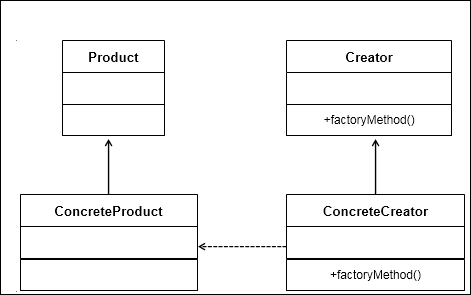
\includegraphics[width=10cm]{figures/factory_pattern.jpg} %NOMBRE DE LA FIGURA y TAMAÑO
    \caption{Arquitectura del patrón de diseño \textit{Factory Pattern}} %PIE DE LA IMAGEN
    \label{factory_pattern}
\end{figure}
 
 \textit{MVC} (patrón de tipo estructural) que se encargue de la gestión tanto de peticiones, como de la identificación de servicios y su respuesta, como se muestra en \ref{mvc_pattern}. \newline 
 
 \begin{figure}[!ht]
    \centering
    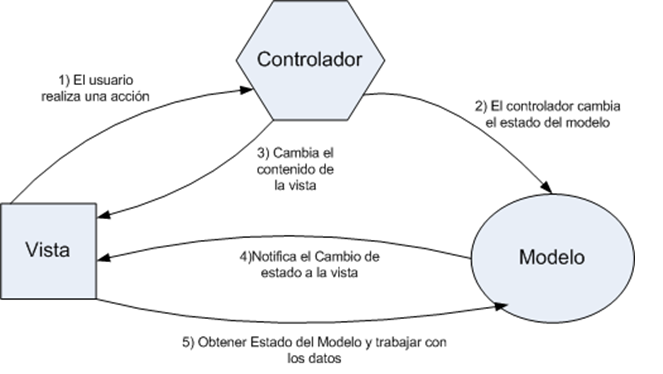
\includegraphics[width=10cm]{figures/mvc_pattern.png} %NOMBRE DE LA FIGURA y TAMAÑO
    \caption{Arquitectura del patrón de diseño \textit{MVC}} %PIE DE LA IMAGEN
    \label{mvc_pattern}
\end{figure}
 
 Los anteriores amalgamados con el \textit{Web Service Broker Pattern} que se encargue de la gestion de servicios web, ubicación de recursos y tipo de resultados, desde una perspectiva más general, como se muestra en la figura \ref{web_service_pattern}.
 
 \begin{figure}[!ht]
    \centering
    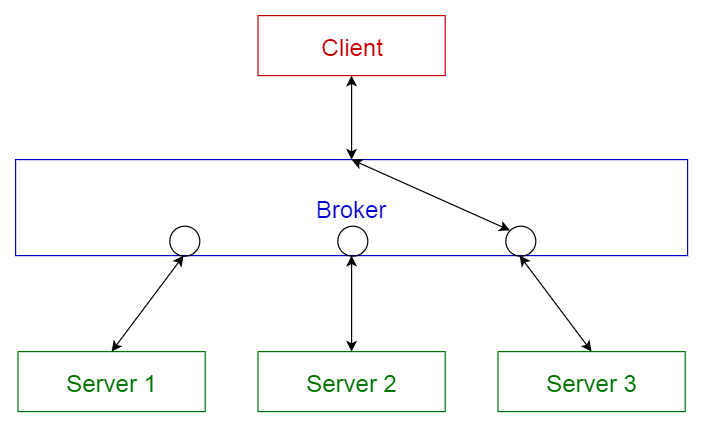
\includegraphics[width=10cm]{figures/web_service_broker_pattern.png} %NOMBRE DE LA FIGURA y TAMAÑO
    \caption{Arquitectura del patrón de diseño \textit{Web Service Broker Pattern}} %PIE DE LA IMAGEN
    \label{web_service_pattern}
\end{figure}


\section{Estado del arte}

\cite{DrJulioSoler} plantea la transferencia de los resultados de investigación entre universidades o instituciones que, aunque las preservan, generan y transmiten, tienen necesidad de realizarlo de manera eficiente y efectiva posible, produciendo resultados favorables para los involucrados. Al mismo tiempo, se señala la importancia de la representación de un dominio adecuado de la gestión de la información científica definido mediante una ontología, sobre un software licenciado para la gestión de contenidos (CMS\footnote{Content Management System}, Sistema de administración de contenidos) y con contenido enriquecido semánticamente. \newline

La Referencia\cite{LaReferencia} \footnote{Disponible en: http://www.lareferencia.info/es/} (Red de Repositorios de Acceso Abierto a la Ciencia) brinda un espacio para la divulgación de la ciencia en Latinoamérica, incluye en su catálogo repositorios de países como Argentina, Brasil, Chile, Colombia, Costa Rica, Ecuador, El Salvador, México y Perú. En los contenidos, los usuarios pueden consultar nodos nacionales, documentos varios, artículos, reportes y  tanto de maestría como de doctorado, cuyas estadísticas generales se muestran en la figura \ref{la-referencia}.

\begin{figure}[!ht]
	\centering
	\fbox{
	\includegraphics[width=12cm]{figures/la_referencia_1.jpg}} %NOMBRE DE LA FIGURA y TAMAÑO
    \caption{Vista principal de LA Referencia} %PIE DE LA IMAGEN
    \label{la-referencia}
\end{figure}

OpenDOAR \footnote{Disponible en: http://v2.sherpa.ac.uk/opendoar/} es un directorio global de repositorios de acceso abierto académico. Permite la identificación, navegación y búsqueda de repositorios, en función de una serie de características, como la ubicación, el software o el tipo de material que se posee. Mediante este sitio web se consultaron repositorios institucionales en España y Estados Unidos de América con el objetivo de identificar aquellos que cuentan con servicios de consultas semánticas. Las figuras \ref{opendoar_estadisticas_1} y \ref{opendoar_estadisticas_2} muestran sus estadisticas globales al día 5 de marzo de 2019.\newline

\begin{figure}[!ht]
	\centering
	\fbox{
	\includegraphics[width=12cm]{figures/opendoar_3.jpg}} %NOMBRE DE LA FIGURA y TAMAÑO
    \caption{Repositorios por país en OpenDOAR} %PIE DE LA IMAGEN
    \label{opendoar_estadisticas_1}
\end{figure}

\begin{figure}[!ht]
	\centering
	\fbox{
	\includegraphics[width=12cm]{figures/opendoar_4.jpg}} %NOMBRE DE LA FIGURA y TAMAÑO
    \caption{Repositorios por lenguaje y tipo de software en OpenDOAR} %PIE DE LA IMAGEN
    \label{opendoar_estadisticas_2}
\end{figure}

El cuadro \ref{repositorios_URL} muestra los repositorios consultados y su ubicación actual.\newline

\begin{table}[htbp]
    \begin{center}
    \begin{tabular}{| p{6.0cm}| p{8.0cm} |}
    \hline
    \centering \textbf{Repositorio} & \textbf{URL} \\
    \hline \hline
    Sistema Nacional de Repositorios Digitales - SNRD (Argentina) & \textit{http://repositoriosdigitales.mincyt.gob.ar/} \\ \hline
    Repositorio CONICYT (Chile) & \textit{http://repositorio.conicyt.cl/} \\ \hline
    Portal Brasileño de Publicaciones Científicas y Acceso Abierto - OASIS (Brasil) & \textit{http://oasisbr.ibict.br/} \\ \hline
    Sistema Nacional de Acceso Abierto al Conocimiento - SNAAC (Colombia) & \textit{http://190.242.114.6:8080/web/guest/inicio} \\ \hline
    Acceso Libre a Información Científica para la Innovación - ALICIA
(Perú) & \textit{https://alicia.concytec.gob.pe/} \\ \hline
    Repositorio Nacional - RN (México) & \textit{https://www.repositorionacionalcti.mx/} \\ \hline
    Red Mexicana de Repositorios Institucionales - REMERI (México) & \textit{http://www.remeri.org.mx/portal/index.html} \\ \hline
    \end{tabular}
    \caption{Ubicación de repositorios consultados.}
    \label{repositorios_URL}
    \end{center}
\end{table}

El cuadro \ref{repositorios_URL_estadisticas} muestra las características generales con las que cuenta cada repositorio consultado a través de LA Referencia.\newline

\begin{table}[htbp]
    \begin{center}
    \begin{tabular}{| p{6.5cm}| p{2.1cm} | p{2.2cm} | p{2.2cm} |}
    \hline
    \centering \textbf{Repositorio} & \textbf{Documentos} & \textbf{Instituciones} & \textbf{Repositorios} \\
    \hline \hline
    Sistema Nacional de Repositorios Digitales - SNRD (Argentina) & 176,927 & 30 & 31 \\ \hline
    Repositorio CONICYT (Chile) & 99,026 & 5,077 & - \\ \hline
    Portal Brasileño de Publicaciones Científicas y Acceso Abierto - OASIS (Brasil) & 2,405,456 & 1,000 & - \\ \hline
    Sistema Nacional de Acceso Abierto al Conocimiento - SNAAC (Colombia) & 116,041 & 45 & 28 \\ \hline
    Acceso Libre a Información Científica para la Innovación - ALICIA (Perú) & 836,582 & 233 & 0 \\ \hline
    Repositorio Nacional - RN (México) & 59,792 & 80 & 87 \\ \hline
    Red Mexicana de Repositorios Institucionales - REMERI (México) & 483,603 & 67 & 98 \\ \hline
    \end{tabular}
    \caption{Estadísticas generales de los repositorios consultados.}
    \label{repositorios_URL_estadisticas}
    \end{center}
\end{table}

El cuadro \ref{repositorios_URL_busquedas} muestra el tipo de servicios de búsqueda disponibles para los usuarios, donde se debe resaltar que los atributos recurrentes para las búsquedas básicas son: título y autor; mientras que en el caso de las avanzadas, el número de parámetros de búsqueda van de cuatro a doce. Finalmente, se pudo identificar que, ninguno de los repositorios consultados cuenta con el servicio de búsquedas semánticas.\newline

\begin{table}[htbp]
    \begin{center}
    \begin{tabular}{| p{6.5cm}| p{1.2cm} | p{1.2cm} | p{1.2cm} | p{1.2cm} | p{1.2cm} |}
    \hline
    \centering \textbf{Repositorio} & \textbf{Básica} & \textbf{No. Atributos} & \textbf{Avanzada} & \textbf{No. Atributos} & \textbf{Semántica} \\
    \hline \hline
    Sistema Nacional de Repositorios Digitales - SNRD (Argentina) & \Checkmark & 2 & \Checkmark & 4 & \XSolidBrush\\ \hline
    Repositorio CONICYT (Chile) & \Checkmark & 6 & \Checkmark & 1 & \XSolidBrush \\ \hline
    Portal Brasileño de Publicaciones Científicas y Acceso Abierto - OASIS (Brasil) & \Checkmark & 3 & \Checkmark & 7 & \XSolidBrush \\ \hline
    Sistema Nacional de Acceso Abierto al Conocimiento - SNAAC (Colombia) & \Checkmark & - & \Checkmark & 9 & \XSolidBrush \\ \hline
    Acceso Libre a Información Científica para la Innovación - ALICIA (Perú) & \Checkmark & 6 & \Checkmark & 9 & \XSolidBrush \\ \hline
    Repositorio Nacional - RN (México) & \Checkmark & - & \Checkmark & 12 & \XSolidBrush \\ \hline
    Red Mexicana de Repositorios Institucionales - REMERI (México) & \Checkmark & - & \XSolidBrush & 0 & \XSolidBrush \\ \hline
    \end{tabular}
    \caption{Tipos de búsquedas y atributos \textit{Dublin Core} en los repositorios consultados}
    \label{repositorios_URL_busquedas}
    \end{center}
\end{table}

Las figuras de la \ref{snrd-1} a la \ref{alicia-1} muestran las páginas inciales de los repositorios consultados y sus módulos de busqueda.

\begin{figure}[!ht]
	\centering
	\fbox{
	\includegraphics[width=12cm]{figures/repositorio_snrd_arg_1.jpg}}
    \caption{Vista del portal del Sistema Nacional de Repositorios Digitales} %PIE DE LA IMAGEN
    \label{snrd-1}
\end{figure}

\begin{figure}[!ht]
	\centering
	\fbox{
	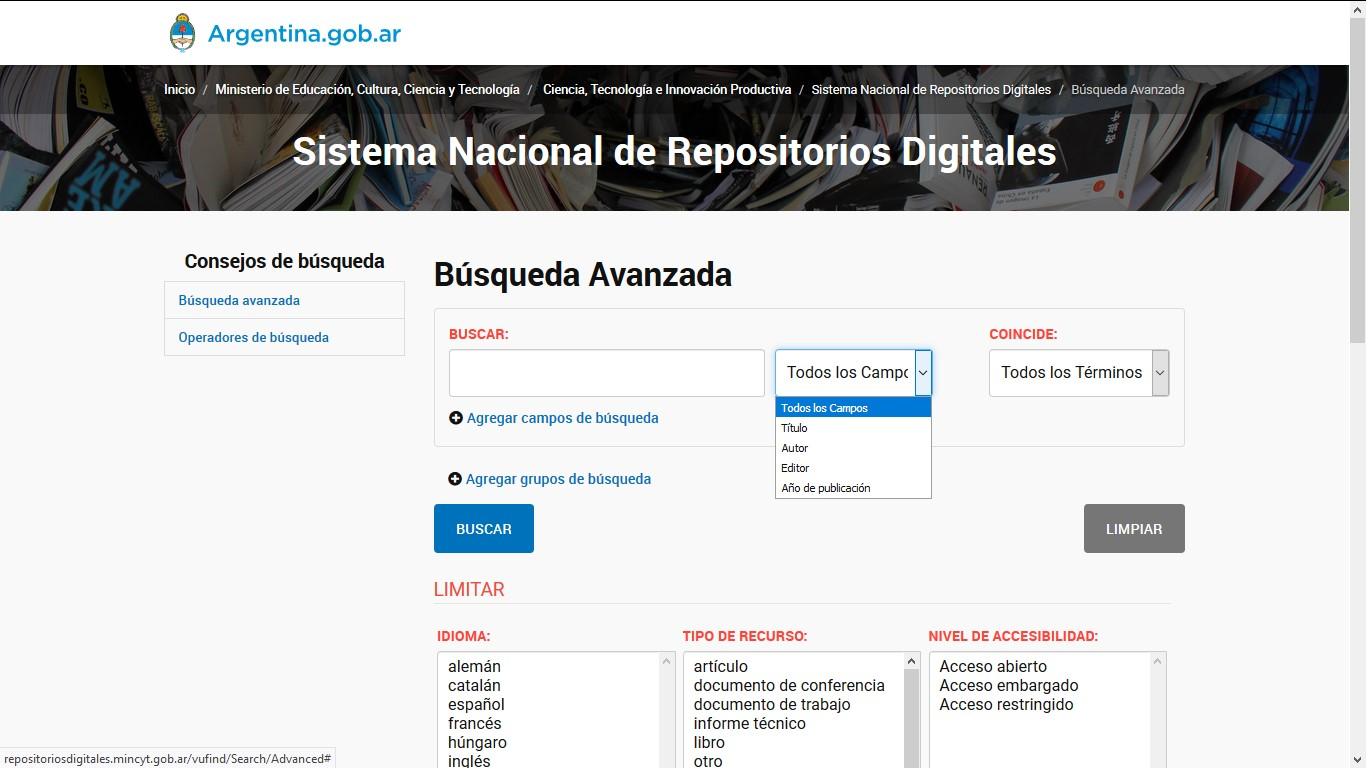
\includegraphics[width=12cm]{figures/repositorio_snrd_arg_2.jpg}} %NOMBRE DE LA FIGURA y TAMAÑO
    \caption{Vista del panel de búsquedas en el SNRD} %PIE DE LA IMAGEN
    \label{snrd-2}
\end{figure}

\begin{figure}[!ht]
	\centering
	\fbox{
	\includegraphics[width=12cm]{figures/repositorio_snrd_br_1.jpg}} %NOMBRE DE LA FIGURA y TAMAÑO
    \caption{Vista del portal Brasileño de Publicaciones Científicas y Acceso Abierto - oasisbr} %PIE DE LA IMAGEN
    \label{oasisbr-1}
\end{figure}

\begin{figure}[!ht]
	\centering
	\fbox{
	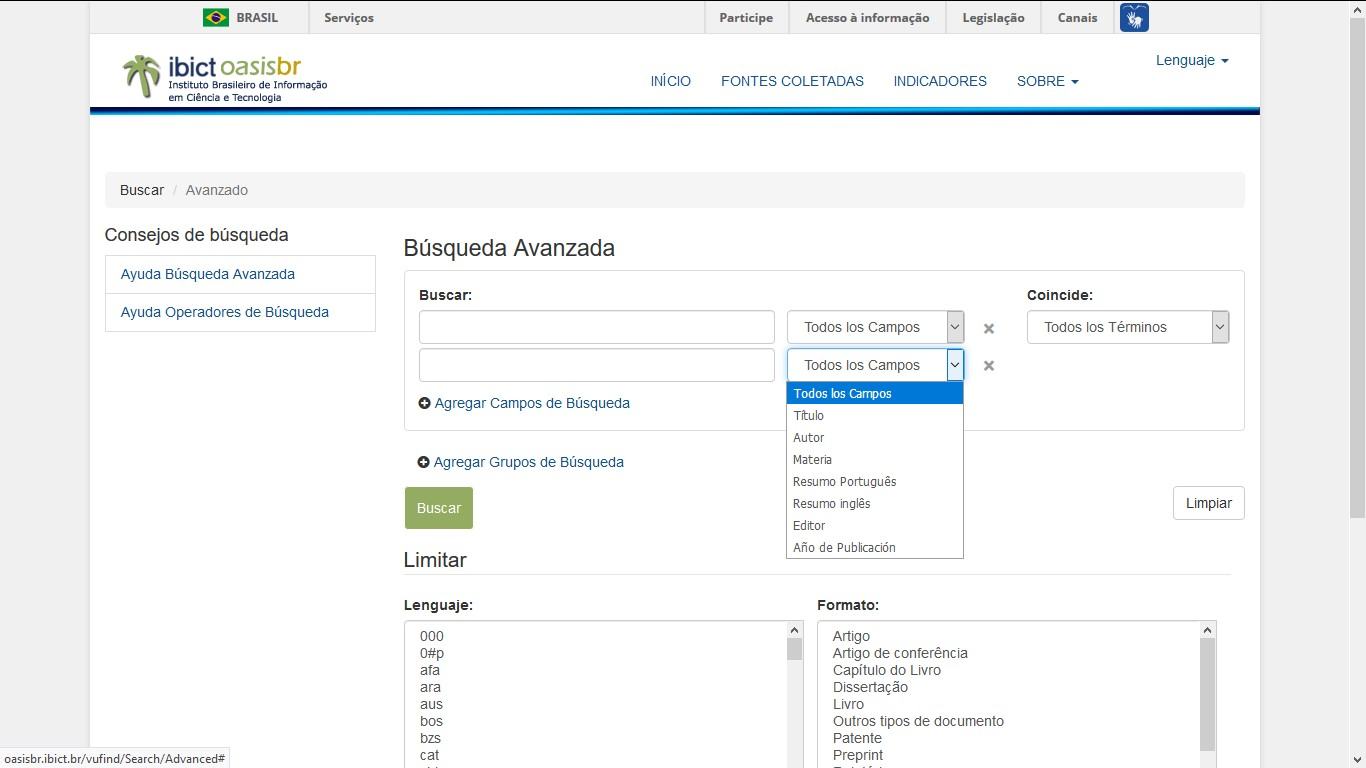
\includegraphics[width=12cm]{figures/repositorio_snrd_br_2.jpg}} %NOMBRE DE LA FIGURA y TAMAÑO
    \caption{Vista del panel de búsquedas en oasisbr} %PIE DE LA IMAGEN
    \label{oasisbr-2}
\end{figure}

\begin{figure}[!ht]
	\centering
	\fbox{
	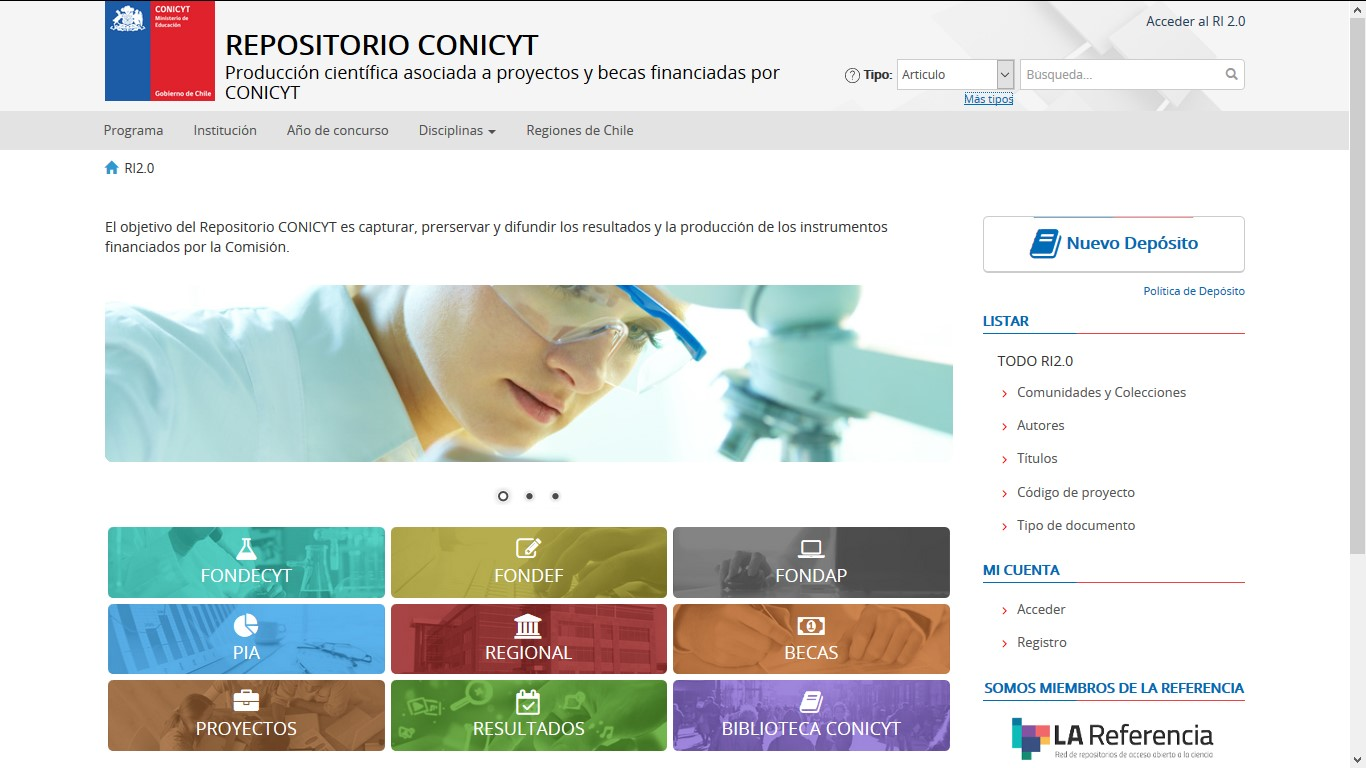
\includegraphics[width=12cm]{figures/repositorio_conicyt_chi_1.jpg}} %NOMBRE DE LA FIGURA y TAMAÑO
    \caption{Vista del portal Sistema de Información Científica} %PIE DE LA IMAGEN
    \label{ri2.0-1}
\end{figure}

\begin{figure}[!ht]
	\centering
	\fbox{
	\includegraphics[width=12cm]{figures/repositorio_conicyt_chi_3.jpg}} %NOMBRE DE LA FIGURA y TAMAÑO
    \caption{Vista del panel de búsquedas en RI2.0} %PIE DE LA IMAGEN
    \label{ri2.0-2}
\end{figure}

\begin{figure}[!ht]
	\centering
	\fbox{
	\includegraphics[width=12cm]{figures/repositorio_conicyt_chi_2.jpg}} %NOMBRE DE LA FIGURA y TAMAÑO
    \caption{Vista del panel de búsquedas avanzadas en RI2.0} %PIE DE LA IMAGEN
    \label{ri2.0-3}
\end{figure}

\begin{figure}[!ht]
	\centering
	\fbox{
	\includegraphics[width=12cm]{figures/repositorio_snaac_1.jpg}} %NOMBRE DE LA FIGURA y TAMAÑO
    \caption{Vista del Sistema Nacional de Acceso Abierto al Conocimiento} %PIE DE LA IMAGEN
    \label{snaac-1}
\end{figure}

\begin{figure}[!ht]
	\centering
	\fbox{
	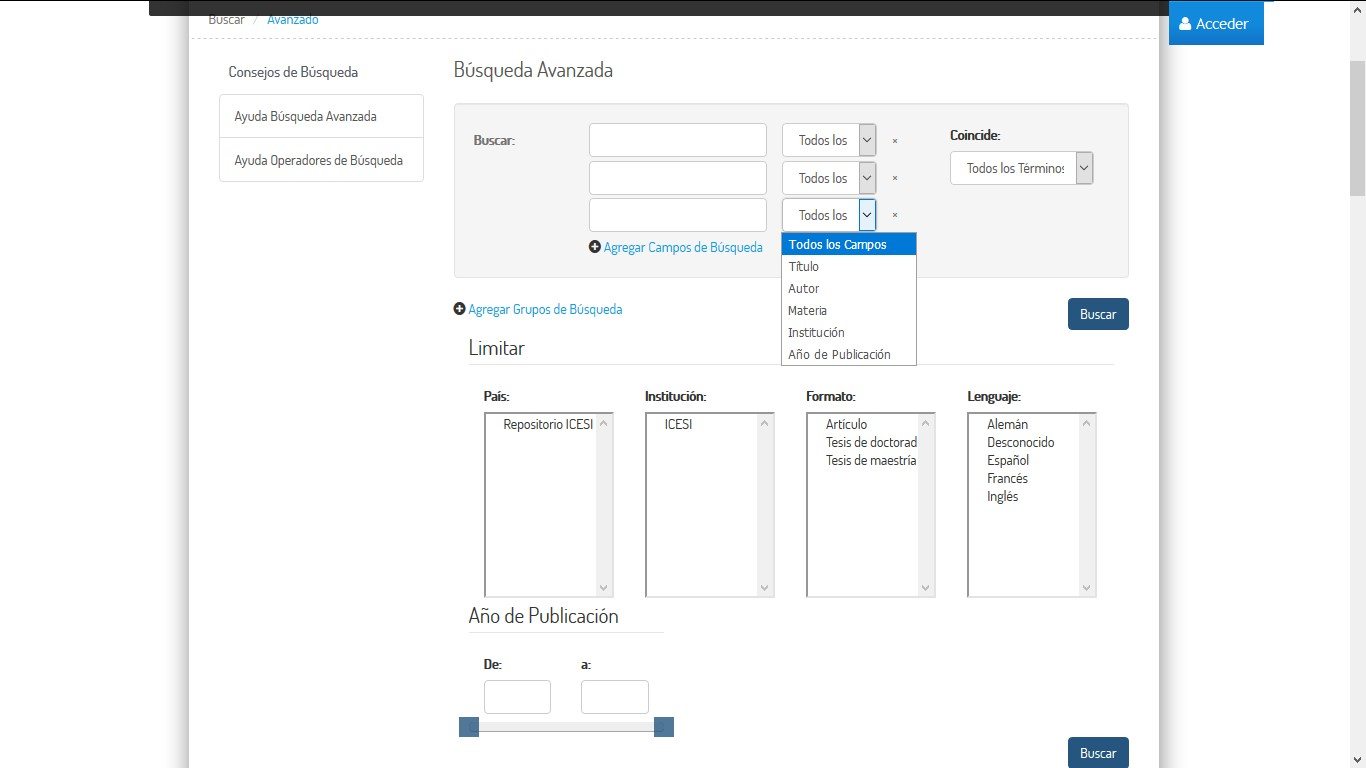
\includegraphics[width=12cm]{figures/repositorio_snaac_2.jpg}} %NOMBRE DE LA FIGURA y TAMAÑO
    \caption{Vista del panel de búsquedas en SNAAC} %PIE DE LA IMAGEN
    \label{snaac-2} 
\end{figure}

\begin{figure}[!ht]
	\centering
	\fbox{
	\includegraphics[width=12cm]{figures/repositorio_alicia_peru_1.jpg}} %NOMBRE DE LA FIGURA y TAMAÑO
    \caption{Vista del portal de Acceso Libre a Información Científica para la Innovación} %PIE DE LA IMAGEN
    \label{alicia-1}
\end{figure}

c